\documentclass[%
  crop,%
  tikz,%
  multi=false%
]{standalone}%
\usepackage[utf8]{luainputenc}%
\usepackage[no-math]{fontspec}%
\defaultfontfeatures{%
  Numbers={OldStyle,Proportional},%
  Ligatures=TeX,%
  Extension=.ttf,%
}%
\setmainfont[%
  UprightFont=*-Regular,%
  ItalicFont=*-Italic,%
  BoldFont=*-Bold,%
  BoldItalicFont=*-BoldItalic,%
]{Raleway}%
\setsansfont[%
  UprightFont=*-Regular,%
  ItalicFont=*-Italic,%
  BoldFont=*-Bold,%
  BoldItalicFont=*-BoldItalic,%
]{Raleway}%
\usepackage[frenchmath]{mathastext}%
\usepackage{amsmath}%
\usepackage{amssymb}%
\usepackage{mathrsfs}%
\usepackage{mathtools}%
\usepackage{siunitx}%
\usepackage[siunitx]{circuitikz}%
\usetikzlibrary{calc,backgrounds,arrows.meta,patterns,positioning}%
\ctikzset{bipoles/length=1.2cm}%

% Colors
\usepackage{xcolor}%
\definecolor{RoseauGreen}{HTML}{cad40e}%
\definecolor{RoseauGrey}{HTML}{adb9cb}%
\definecolor{RoseauBlue}{HTML}{234e83}%

\DeclareMathOperator{\sign}{sign}%

% Sets
\let\C\relax
\newcommand{\R}{\ensuremath{\mathbb{R}}} % Real
\newcommand{\N}{\ensuremath{\mathbb{N}}} % Natural
% \newcommand{\C}{\ensuremath{\mathbb{C}}} % Complexes
\newcommand{\B}{\ensuremath{\mathscr{B}}} % Electrical buses
\newcommand{\Ch}{\ensuremath{\mathscr{C}}} % Loads
\renewcommand{\L}{\ensuremath{\mathscr{L}}} % Lines
\renewcommand{\P}{\ensuremath{\mathscr{P}}} % Phases

% Phases
\newcommand{\arm}{\ensuremath{\mathrm{a}}}%
\newcommand{\brm}{\ensuremath{\mathrm{b}}}%
\newcommand{\crm}{\ensuremath{\mathrm{c}}}%
\newcommand{\nrm}{\ensuremath{\mathrm{n}}}%
\newcommand{\grm}{\ensuremath{\mathrm{g}}}%
\newcommand{\abrm}{\ensuremath{\mathrm{ab}}}%
\newcommand{\bcrm}{\ensuremath{\mathrm{bc}}}%
\newcommand{\carm}{\ensuremath{\mathrm{ca}}}%
\newcommand{\anrm}{\ensuremath{\mathrm{an}}}%
\newcommand{\bnrm}{\ensuremath{\mathrm{bn}}}%
\newcommand{\cnrm}{\ensuremath{\mathrm{cn}}}%
\newcommand{\agrm}{\ensuremath{\mathrm{ag}}}%
\newcommand{\bgrm}{\ensuremath{\mathrm{bg}}}%
\newcommand{\cgrm}{\ensuremath{\mathrm{cg}}}%
\newcommand{\ngrm}{\ensuremath{\mathrm{ng}}}%
\newcommand{\abcrm}{\ensuremath{\mathrm{abc}}}%
\newcommand{\abcnrm}{\ensuremath{\mathrm{abcn}}}%

% Transformer
\newcommand{\Xrm}{\ensuremath{\mathrm{X}}}%
\newcommand{\Yrm}{\ensuremath{\mathrm{Y}}}%
\newcommand{\Zrm}{\ensuremath{\mathrm{Z}}}%
\newcommand{\xrm}{\ensuremath{\mathrm{x}}}%
\newcommand{\yrm}{\ensuremath{\mathrm{y}}}%
\newcommand{\zrm}{\ensuremath{\mathrm{z}}}%
\newcommand{\Arm}{\ensuremath{\mathrm{A}}}%
\newcommand{\Brm}{\ensuremath{\mathrm{B}}}%
\newcommand{\Crm}{\ensuremath{\mathrm{C}}}%
\newcommand{\Nrm}{\ensuremath{\mathrm{N}}}%

% Indices or exponents
\newcommand{\cons}{\ensuremath{\mathrm{cons.}}}%
\renewcommand{\prod}{\ensuremath{\mathrm{prod.}}}%
\newcommand{\theo}{\ensuremath{\mathrm{th.}}}%
\newcommand{\const}{\ensuremath{\mathrm{const.}}}%

% Variables
\newcommand{\umax}{\ensuremath{U^{\max}}}%
\newcommand{\umaxnorm}{\ensuremath{U^{\max\,\text{norm.}}}}%
\newcommand{\umin}{\ensuremath{U^{\min}}}%
\newcommand{\uminnorm}{\ensuremath{U^{\min\,\text{norm.}}}}%
\newcommand{\unom}{\ensuremath{U^{\text{nom.}}}}%
\newcommand{\unomnorm}{\ensuremath{U^{\text{nom.}\,\text{norm.}}}}%
\newcommand{\uup}{\ensuremath{U^{\text{up}}}}%
\newcommand{\uupnorm}{\ensuremath{U^{\text{up}\,\text{norm.}}}}%
\newcommand{\uupprime}{\ensuremath{U^{\text{up}\,\prime}}}%
\newcommand{\udown}{\ensuremath{U^{\text{down}}}}%
\newcommand{\udownnorm}{\ensuremath{U^{\text{down}\,\text{norm.}}}}%
\newcommand{\udownprime}{\ensuremath{U^{\text{down}\,\prime}}}%
\newcommand{\smax}{\ensuremath{S^{\max}}}%
\newcommand{\pmax}{\ensuremath{P^{\max}}}%
\newcommand{\sproj}{\ensuremath{\underline{S^{\text{proj.}}}}}%
%

\begin{document}
\ctikzset{european, straight voltages, cute inductors, bipoles/length=1cm, voltage shift=0.5mm}%
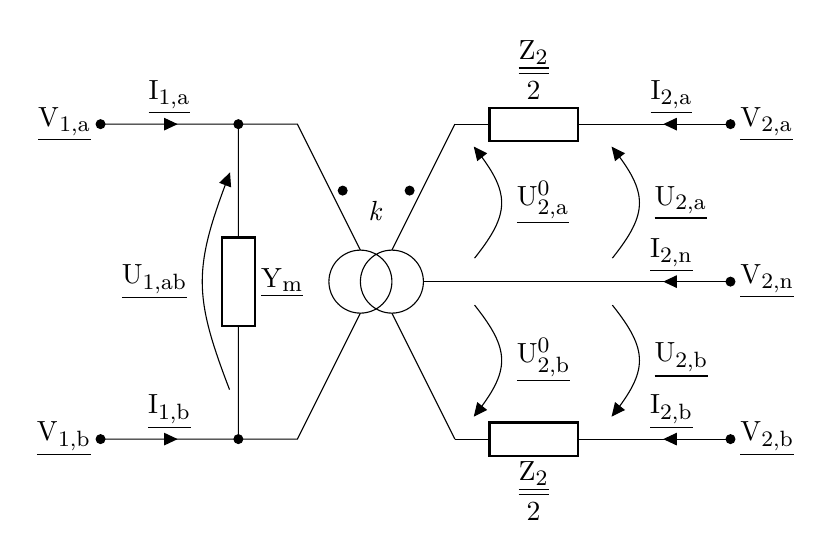
\begin{tikzpicture}[%
    show background rectangle,%
    tight background,%
    background rectangle/.style={fill=white}%
  ]
  % Version multifilaire

  %
  % Définitions
  %
  % No European transformer in circuitikz [BV, 17/07/2023]
  \tikzset{
    transformer/.pic={
      \draw (-0.2,0) circle[radius=0.4] (0.2,0) circle[radius=0.4];
    },
  }
  \pgfmathsetmacro{\xl}{0};%
  \pgfmathsetmacro{\xy}{1.75};%
  \pgfmathsetmacro{\xlt}{2.5};%
  \pgfmathsetmacro{\xrt}{4.5};%
  \pgfmathsetmacro{\xz}{6.5};%
  \pgfmathsetmacro{\xm}{8};%
  \pgfmathsetmacro{\xtransformer}{0.5*(\xlt+\xrt)};%
  \pgfmathsetmacro{\xtransformerm}{\xtransformer-1};%
  \pgfmathsetmacro{\xtransformerp}{\xtransformer+1};%

  \pgfmathsetmacro{\yb}{0};%
  \pgfmathsetmacro{\yn}{2};%
  \pgfmathsetmacro{\ya}{4};%
  \pgfmathsetmacro{\yt}{0.5*(\ya+\yb)};%

  %
  % Dessin
  %
  % Transformer
  \pic[local bounding box=T] at (\xtransformer,\yt) {transformer};%
  \node[above=0.25cm] at (T.north) {$k$};%

  % Tensions amont
  \node[left] at (\xl,\ya) {$\underline{V_{1,\arm}}$};
  \node[left] at (\xl,\yb) {$\underline{V_{1,\brm}}$};

  % Tensions aval
  \node[right] at (\xm,\ya) {$\underline{V_{2,\arm}}$};
  \node[right] at (\xm,\yb) {$\underline{V_{2,\brm}}$};
  \node[right] at (\xm,\yn) {$\underline{V_{2,\nrm}}$};

  % Câbles principaux
  % A
  \draw (\xl,\ya) to[short,*-*,i=$\underline{I_{1,\arm}}$]
  (\xy,\ya) to[short] (\xtransformerm,\ya) to[short] node[near start,above=0.25cm,circ] {} (T);%
  \draw (\xtransformerp,\ya) to[short] node[near start,above=0.25cm,circ] {} (T);%
  \draw (\xtransformerp,\ya) -- (\xrt,\ya) to[generic, l=$\dfrac{\underline{Z_2}}{2}$, label distance=6pt, -]
  (\xz,\ya) to[short,-*,i<=$\underline{I_{2,\arm}}$] (\xm,\ya);%

  % B
  \draw (\xl,\yb) to[short,*-*,i=$\underline{I_{1,\brm}}$]
  (\xy,\yb) to[short] (\xtransformerm,\yb) to[short] (T);%
  \draw (\xtransformerp,\yb) to[short] (T);%
  \draw (\xtransformerp,\yb) -- (\xrt,\yb) to[generic, l_=$\dfrac{\underline{Z_2}}{2}$, -]
  (\xz,\yb) to[short,-*,i<=$\underline{I_{2,\brm}}$] (\xm,\yb);%

  % Neutre
  \draw (T.east) to[short] (\xtransformerp,\yn) -- (\xz,\yn) to[short,-*,i<=$\underline{I_{2,\nrm}}$] (\xm,\yn);%

  % Ym
  \draw (\xy,\ya) to[generic, l=$\underline{Y_{\mathrm{m}}}$, v<=$\underline{U_{1,\abrm}}$, -] (\xy,\yb);%

  % Tensions
  \draw (\xz,\ya) to[open, v^<=$\underline{U_{2,\arm}}$] (\xz,\yn);%
  \draw (\xz,\yb) to[open, v<=$\underline{U_{2,\brm}}$] (\xz,\yn);%
  \pgfmathsetmacro{\xr}{\xrt + 0.25};%
  \draw (\xr,\ya) to[open, v^<=$\underline{U_{2,\arm}^0}$] (\xr,\yn);%
  \draw (\xr,\yb) to[open, v<=$\underline{U_{2,\brm}^0}$] (\xr,\yn);%

\end{tikzpicture}
\end{document}
% Local Variables:
% mode: latex
% TeX-engine: luatex
% TeX-source-correlate-method-active: synctex
% ispell-local-dictionary: "british"
% coding: utf-8
% LaTeX-indent-level: 2
% fill-column: 120
% End:
